\section{Formalisation théorique}\label{sec:contrib:asteroid:theorie}
Dans cette section, nous présentons les fondamentaux théoriques pour permettre l'intégration d'un support persistant relationnel dans Astral et dans notre architecture. Tout d'abord, nous présentons en détail les différents motifs d'évolutions des données persistantes ou temps réel. Ces motifs auront des impacts sur le schéma de la base de donnée utilisé pour la persistance que nous présentons par la suite. Enfin, nous décrivons comment une relation persistante sera représentée en tant que relation temporelle.

\subsection{Dynamique des données}
Dans un système, nous avons vu que les données peuvent être persistantes ou temps réel. Nous remarquons aussi que les données évoluent suivant des schémas différents qui vont influencer la manière de les manipuler par la suite. Notamment, cela a un impact non négligeable sur le schéma utilisé dans le SGBD relationnel pour le support de persistance.

Par définition, la persistance d'une donnée implique le fait de stocker l'information sur un support. Sa mise à jour sur ce support est une opération considérée comme lente\footnote{Cette lenteur a permit la création des SGFD à la fin des années 90.}. Ainsi, il sera difficile de supposer possible le fait d'avoir une représentation physique acceptable de toutes les données du système.

Les données persistantes sont considérés en quatre dynamiques divisées en deux catégories. Tout d'abord, celles que nous qualifions de meta-données qui sont rassemblés dans des catalogues (donc, des relations persistantes). Celle-ci est composé de deux classes de dynamiques :
\begin{itemize}
	\item[\textbf{Statique}] Cette meta-donnée ne changera jamais par essence. Son utilisation en interrogation continue sera similaire à une relation temporelle $R$ figée : $R^{t_0}$. Le numéro de série d'un équipement est une information qui par nature est immuable.
	\item[\textbf{Stable}] Cette meta-donnée est considéré la plupart du temps comme figée. Elle n'est toutefois pas immuable par essence et peut subir des modifications. Bien que son utilisation soit avant-tout une interrogation instantannée, son utilisation en interrogation continue est une relation temporelle $R$ n'ayant subit aucune manipulation temporelle. Un paramètre de configuration d'un équipement du réseau local est considéré comme stable.
\end{itemize}

La deuxième catégorie rassemble les données évoluant en temps réel. Ces données sont issus de flux de données. Elles peuvent posséder deux dynamiques :
\begin{itemize}
	\item[\textbf{Périodique}] L'historique de cette donnée forme un flux régulier. Son interrogation continue passe par l'application d'une fenêtre dont le contenu n'est pas limité à un \textit{batch}. En effet, la régularité induite par cette donnée implique qu'il est plus important d'observer son évolution plutôt que sa valeur présente. Le relevé des débits d'une carte réseau constitue une donnée périodique.
	\item[\textbf{Imprévisible}] Cette donnée n'a pas de motif d'évolution défini a priori. Son comportement incontrôlable fait que chaque nouvelle donnée du flux a son importante. Son utilisation en requête continue est donc faite par l'application d'une fenêtre $[B]$ décrivant le dernier \textit{batch}. La notification de l'arrivée d'un équipement sur le réseau est imprévisible.
\end{itemize}

Le principe important est le fait que ces classes de dynamiques sont manipulables grâce à l'algèbre. Il est possible de figer une donnée à un instant grâce à la manipulation temporelle. Il est possible de former un flux de changement à partir d'une relation stable. De plus, elle traduit une certaine qualité de la donnée car si nous utilisons une donnée d'une classe comme une autre alors nous perdrons de la qualité.
\begin{example}
	Si nous récupérons les notifications d'arrivée des équipements sur le réseau de manière périodique, nous perdons de la qualité en terme de ponctualité. De même si nous considérons un paramètre de configuration comme statique. A l'inverse, nous introduisons du bruit si nous interrogeons de manière périodique la configuration du routeur de la passerelle d'accès à internet.
\end{example}

Il est important de voir que ces classes nous permettent d'imaginer les mécanismes les plus adaptés pour collecter les données. Toutefois, si un mécanisme n'est pas disponible et qu'un autre est utilisé\footnote{\textit{push} absent $\im$ remplacement par un \textit{pull} régulier}, cela nous permet d'en analyser rapidement les conséquences. La figure~\ref{fig:contrib:asteroid:theorie:dynamics} montre des transformations possibles entre les dynamiques grâce à l'algèbre Astral. Les méta-données sont représenté par des relations temporelles $R$ et les données temps-réelles sont des flux non-partitionnables $S$.

\begin{figure}[ht]
    \centering
\scalebox{0.8}{
\tikzstyle{dynamics}=[ellipse,minimum width=3cm,minimum height=1cm,draw=blue!50,fill=blue!20,thick]
\begin{tikzpicture}[>=stealth,->,shorten >=2pt,thick,bend angle=20, node distance=7cm]
\node (relation) {Méta-données};
\node (flux) [below of=relation,node distance=3cm] {Temps-réel};

\node[dynamics] (static) [right of=relation,node distance=4cm]{Statique};
\node[dynamics] (stable) [right of=static] {Stable};
\node[dynamics] (periodic) [below of=static,node distance=3cm] {Périodique};
\node[dynamics] (event) [right of=periodic] {Imprévisible};

\tikzstyle{every node}=[auto]
\path (stable)      edge    node[above]{$R^{t_0}$} (static);
\path (event)       edge    node[near end,above,sloped]{$S[B]^{\tau_S(0)}$} (static);
\path (periodic)    edge[bend left]    node{$S[B]^{\tau_S(0)}$} (static);
\path (static)      edge[bend left]    node[right]{$\RS{r}(R)$} (periodic);
\path (stable)      edge    node[near end,below,sloped]{$\RS{r}(R)$} (periodic);
\path (event)       edge    node{$\RS{r}(S[B])$} (periodic);

\path (stable)      edge[bend left]    node{$\IS(R)$} (event);
\path (event)      edge[bend left]    node{$S[B]$} (stable);
\end{tikzpicture}
}
\caption{Transformations des différentes dynamiques en Astral}\label{fig:contrib:asteroid:theorie:dynamics}
\end{figure}

\subsection{Schéma physique de la persistance}\label{sec:contrib:asteroid:theorie:schema}
La notion de dynamiques va directement impacter la structure du schéma de la base de donnée. Cette persistance va utilisée pour permettre de stocker et conserver deux catégories de données : le modèle descriptif et les historiques de flux.
\subsubsection{Le schéma descriptif}
Les données que nous avons décrites en tant que meta-données forment une description du système observé. Cette description servira de catalogue lors de l'interrogation du système. Elle contiendra l'ensemble des concepts du systèmes, leurs relations ainsi que leurs propriétés. D'un point de vue conceptuel, celui-ci peut-être structuré comme un schéma entité-relation qui pourra par la suite être traduit en schéma physique normalisé.

Le point important étant que tous les concepts dit observables du système sont des sous-classes de \textit{Monitorable}. Cette classe permet avant tout d'identifier de manière unique chaque entité du système (clé artificielle unique). L'idée étant que toute entité pourra être manipulée de façon uniforme.

\begin{example}
	Dans le cadre du réseau local domestique, nous observons un système composé d'équipements. Ces équipements sont hôtes d'applications pouvant avoir un statut allumé ou éteint. Ils peuvent posséder un numéro de série unique. Ces équipements embarquent une ou plusieurs interfaces réseaux. Celles-ci possèdent une adresse \textit{IP} et \textit{MAC} lui considéré comme unique. Le réseau est composé de liens physiques entre les interfaces réseaux.
	
	Nous avons donc les relations \textit{Devices}, \textit{Applications}, \textit{Interfaces} et \textit{Link} qui sont toutes filles de \textit{Monitorable}. Nous obtenons ainsi le schéma physique présenté en figure~\ref{fig:contrib:asteroid:theorie:model}
	\begin{figure}[ht]
                \centering
		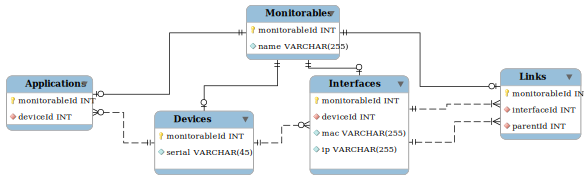
\includegraphics[width=0.9\textwidth]{contrib-asteroid-model}
		\caption{Potentiel schéma descriptif du système : réseau local domestique}\label{fig:contrib:asteroid:theorie:model}
	\end{figure}
\end{example}

\noindent \textbf{Remarque} : Les clés artificielles ont une grande importance dans le cadre des applications d'observation. En effet, du fait du caractère incomplet de l'observation\footnote{soit parce que la donnée n'est pas parvenue au système, soit il n'existe pas de moyen technique pour y accéder}, il est possible d'obtenir des informations sur un équipement par exemple, sans avoir pu obtenir son numéro de série. Des moyens alternatifs d'identifications doivent être mis en place. Par exemple, << \textit{l'équipement qui possède l'adresse IP 192.168.0.1} >> permet d'identifier de manière approximative l'équipement. Les clés artificielles permettent donc de tisser les relations entre les instances en ayant des données partielles. Toutefois, des vérifications d'intégrités devrons être de rigueur pour garder un modèle cohérent.

La différence entre une donnée stable et une donnée statique est le fait qu'il est intéressant de surveiller la modification d'une donnée (par des mécanismes tels que les \textit{triggers}) et en former un flux, qui pourra être potentiellement archivé.

\subsubsection{Les historiques}
Le stockage brut d'un flux $S$ comme relation physique dans le SGBD est difficilement manipulable. Car de ce fait, les données de flux persistées n'ont aucun lien avec le système. Or, toute donnée temps réel concerne une entité du catalogue du système. Et toute donnée temps réel est matérialisé par la relation temporelle $S[\infty]$.

Nous appelons \textit{Volatile} une donnée temps réel. Nous modélisons donc notre persistance des historiques par l'association donnant à partir d'une entité et d'un \textit{volatile}, la relation contenant son historique. D'un point de vue physique, les SGBD supportent mal cette implémentation ce qui fait que ce dernier est en réalité une table contenant un pointeur vers une table qui elle contient l'historique comme montré dans la figure~\ref{fig:contrib:asteroid:theorie:volatile}.


\begin{figure}[ht]
    \centering
    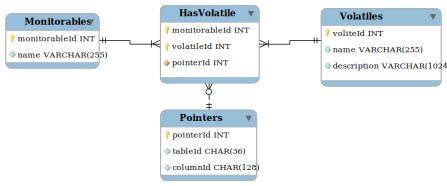
\includegraphics[width=0.8\textwidth]{contrib-asteroid-historians}
    \caption{Représentation physique de l'enregistrement des historiques}\label{fig:contrib:asteroid:theorie:volatile}
\end{figure}

\begin{example}
	La donnée de changement de \textit{status} est une donnée imprévisible aussi bien attachée à un équipement qu'à une application. Lors de l'enregistrement d'un historique de \textit{status} concernant un équipement par exemple, il est donc nécessaire d'insérer un n-uplet dans la relation \textit{TablePointer}, qui permet de déclarer l'historique et un autre dans \textit{HasVolatile} qui permet de lier cette historique à une entité. Si la donnée \textit{status} n'avait pas été déclarée, il est évidemment nécessaire d'insérer un n-uplet dans la relation \textit{Volatile}.
	
	De façon similaire, les relevés de charges processeurs \textit{cpu} sont peuvent être attachés à un équipement ou à une application. Alors que les relevés de débits n'ont de sens que sur les interfaces (ou les liens suivant la modélisation voulue par l'utilisateur).
\end{example}

Il est intéressant de voir que puisque les données temps-réelles ont tendances à être de forte densité, il n'est peut-être pas possible de garantir une fraicheur des données au niveau du support de persistance pour les historiques.

\subsection{Représentation dans Astral}\label{sec:contrib:asteroid:theorie:astral}
Les relations issues d'un SGBD sont manipulables dans Astral du fait de leurs fondations théoriques similaires. Ainsi une relation d'un système relationnel observée de manière continue est assimilable à une relation temporelle. Deux différences majeures subsistent : l'ordre des données et le mode d'interrogation.
\subsubsection{L'ordre d'une relation}
En SGBD, l'ordre n'importe pas jusqu'au moment de l'envoi des données à l'utilisateur (via le mot clé \textit{ORDER BY}). Le système peut en profiter pour modifier l'ordre lors d'opérations de jointures par exemple. Il est important de garder la même notion d'ordre lors de la prise en compte de l'évolution. L'identifiant physique de la relation temporelle induite sera donc par défaut la clé primaire de la relation observée, i.e. son identifiant de monitorable. Ainsi, nous gardons le même identifiant, et l'ordre est conservé lors des opérations.

\subsubsection{Le mode d'interrogation}
Afin d'être capable de représenter une relation temporelle dans \textit{Astronef}, il est nécessaire de pouvoir surveiller les changements effectués dans la relation. Ceci peut toutefois être coûteux ou impossible suivant les moyens techniques disponible dans le SGBD manipulé. Ainsi, pour être capable de représenter la relation telle que nous l'obtenons dans Astronef par la suite, nous utilisons un opérateur de manipulation du temps. Ce qui nous permet d'obtenir, comme indiqué dans la section~\ref{sec:contrib:astral:manipulation}, une mise à jour effective, périodique, à la demande ou inexistante.